\documentclass[aspectratio=169,usenames,dvipsnames]{beamer}
\usepackage{preamble}
\title{Coding for Humanities, week 5}

\begin{document}

\begin{frame}
 \titlepage
\end{frame}

\begin{frame}{Last week}
    Midterm
    
    \vspace{1em}
    Files \& directories

    \vspace{1em}
    Libraries
\end{frame}

\begin{frame}{Plan for today}
 \tableofcontents
\end{frame}

\section{The Midterm}

\begin{frame}
    \begin{reference}
        \scriptsize\vspace{1em}
        \hfill Source: \url{https://oktop.tumblr.com/post/15352780846}
    \end{reference}
    \begin{columns}[b]
        \column{0.5\linewidth}
            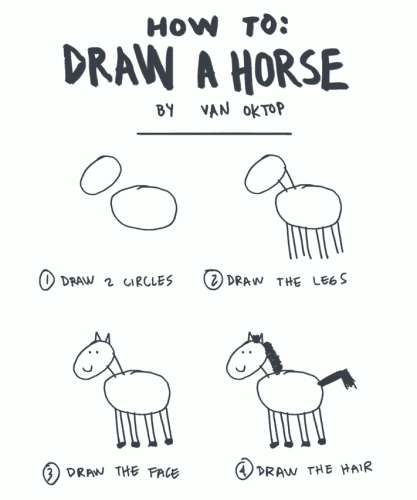
\includegraphics[height=0.9\textheight]{fig/horse1}
        \pause
        \column{0.5\linewidth}
            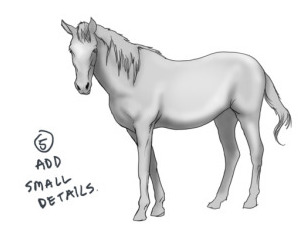
\includegraphics[width=0.9\linewidth]{fig/horse2}
    \end{columns}
\end{frame}

\begin{frame}{The Midterm}
    \begin{itemize}
        \item Solutions on Nestor.
        %\item Common mistakes:
        %    \begin{itemize}
        %        \item \dots
        %        \item \dots
        %    \end{itemize}
        \item Questions? Tomorrow in lab.
    \end{itemize}
\end{frame}

\section{Improving code}
\subsection{Working code}
\frame{\tableofcontents[currentsection]}
\begin{frame}{Working code}
    \begin{definition}
        \structure{Debugging}: identify and fix errors (`bugs') in programs
    \end{definition}

    \pause\vspace{1em}
    \begin{columns}
        \column{0.5\linewidth}
            ``If debugging is the art of removing bugs from programs,
            programming must be the art of inserting them''
            (attributed to Edsger Dijkstra)

            % If you want more effective programmers, you will discover that they should not waste their time debugging, they should not introduce the bugs to start with.
            % (Edsger Dijkstra)
        \column{0.5\linewidth}
            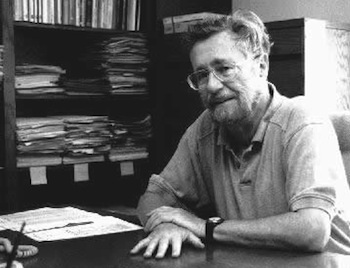
\includegraphics[height=0.5\textheight]{fig/dijkstra}

            \vspace{1em}
            Interview: \url{https://youtu.be/mLEOZO1GwVc}
    \end{columns}
\end{frame}


\begin{frame}
    % On two occasions I have been asked, --- "Pray, Mr. Babbage, if you put
    % into the machine wrong figures, will the right answers come out?" In one
    % case a member of the Upper, and in the other a member of the Lower House
    % put this question. I am not able rightly to apprehend the kind of
    % confusion of ideas that could provoke such a question.

    % Charles Babbage, Passages from the Life of a Philosopher (1864), ch. 5:
    % "Difference Engine No. 1"

    % \pause\vspace{1em}
    % The programmer, like the poet, works only slightly removed from pure
    % thought-stuff. He builds his castles in the air, from air, creating by
    % exertion of the imagination. Few media of creation are so flexible, so
    % easy to polish and rework, so readily capable of realizing grand
    % conceptual structures....
    % Yet the program construct, unlike the poet's words, is real in the sense
    % that it moves and works, producing visible outputs separate from the
    % construct itself. [...] The magic of myth and legend has come true in our
    % time. One types the correct incantation on a keyboard, and a display
    % screen comes to life, showing things that never were nor could be.
    % Fred Brooks (1975) The Mythical Man-Month: Essays on Software Engineering
    % p. 7

    % \pause\vspace{1em}
    % And programming computers was so fascinating. You create your own little
    % universe, and then it does what you tell it to do.
    % Vint Cerf, a "father of the internet," quoted in "Your Life: Vinton Cerf"
    % interview with David Frank in AARP Bulletin (December 2016, Vol. 57, No.
    % 10, p. 28.)

    \begin{columns}
        \column{0.7\linewidth}
    Maurice Wilkes discovers debugging in 1949:

    \vspace{1em}
    \begin{quote}\normalfont
    ``As soon as we started programming, we found to our surprise that it
    wasn't as easy to get programs right as we had thought. Debugging had to be
    discovered. I can remember the exact instant when I realized that a large
    part of my life from then on was going to be spent in finding mistakes in
    my own programs.''
    \end{quote}
        \column{0.3\linewidth}
    \end{columns}
    % \pause\vspace{1em}
    % ``Everyone knows that debugging is twice as hard as writing a program in
    % the first place. So if you're as clever as you can be when you write it,
    % how will you ever debug it?'' (Brian Kernighan)
\end{frame}


\begin{frame}{Common errors}
    \begin{description}[AttributeError]
        \item[SyntaxError] unclosed parenthesis, missing comma, colon etc.
        \item[NameError] typo in variable/function
        \item[IndexError] \texttt{seq[n] with n >= len(seq)}
        \item[KeyError] using key not in dict
        \item[AttributeError] \texttt{obj.att}, but obj does not have att
        \item[TypeError] mixing str/int/etc.
        \item[ValueError] generic error: right type, wrong value
        \item[\dots] \dots
    \end{description}
\end{frame}

\begin{frame}[fragile]{Understanding tracebacks}
\begin{definition}
    \structure{Traceback}: the chain of function calls that led to an error.
\end{definition}
\begin{lstlisting}
>>> from collections import Counter
>>> c = Counter('abcdef')
>>> c.most_common('a')
Traceback (most recent call last):
  File "<stdin>", line 1, in <module>
  File "/usr/lib/python3.7/collections/__init__.py", line 584, in most_common
    return _heapq.nlargest(n, self.items(), key=_itemgetter(1))
  File "/usr/lib/python3.7/heapq.py", line 546, in nlargest
    if n >= size:
TypeError: '>=' not supported between instances of 'str' and 'int'
\end{lstlisting}
\pause
First step: \structure{locate} the root cause.
Typically somewhere in your own code \dots
\end{frame}

\begin{frame}{General strategy}
    The most effective debugging tool is still careful thought, coupled with
    judiciously placed print statements. (Brian Kernighan)
    
    \pause\vspace{1em}
    Go through each line of code \dots
    \begin{itemize}
        \item Think like the computer: \\
            what is happening? \\
            Is it what you intended?
        \item Ask yourself: what is the input and output? \\
            Confirm: print values
        \item Does the problem only occur with particular values? \\
            What is special about them?
        \item For difficult problems, repeat several times.
    \end{itemize}
\end{frame}



\subsection{Good code}
\begin{frame}{Good code: Refactoring}
    Insight: can achieve the same end in many different ways

    \pause
    \begin{definition}
        \structure{Refactoring}: improving code (e.g., readability) \\
            while keeping the same functionality (i.e., behavior).
    \end{definition}

    % FIXME: already mentioned in previous lectures
    % concrete examples, or leave out.
    \begin{itemize}
        \item Clear variable names
        \item Separate steps/functions
        \item Use idioms
    \end{itemize}
\end{frame}

\begin{frame}[fragile]{Example: working code}
\begin{lstlisting}
def clean_tweets(filename):
    with open(filename, encoding='utf8') as infile:
        text = infile.read()
        cleaned_text = ''
        lower_text = text.lower()
        for character in lower_text:
            if character not in '!$%^&*()-+={}[]:;"\'|<>,.?/~`':
                cleaned_text += character
        cleaned_list = cleaned_text.split()
        return cleaned_list
\end{lstlisting}
\end{frame}

\begin{frame}[fragile]{Example: re-factored}
\begin{columns}
\column{0.6\linewidth}
\begin{lstlisting}
def remove_punc(text):
    punctuation = '!$%^&*()-+={}[]:;"\'|<>,.?/~`'
    return ''.join(character for character in text
            if character not in punctuation)

def clean_tweets(filename):
    with open(filename, encoding='utf8') as infile:
        text = infile.read()
    cleaned_text = remove_punc(text.lower())
    tokens = cleaned_text.split()
    return tokens
\end{lstlisting}
\column{0.4\linewidth}
\begin{itemize}
\item Separate function for punctuation
\item More efficient punctuation elimination
\item Limit scope of \textcolor{blue}{\texttt{with}}
\item Renamed \textcolor{blue}{\texttt{cleaned\_list}} \\
    to \textcolor{blue}{\texttt{tokens}}
\end{itemize}
\end{columns}
\end{frame}

\begin{frame}{Code style guides}
    \begin{reference}
        PEP-0008: coding conventions for Python code.
        \url{https://www.python.org/dev/peps/pep-0008/}
    \end{reference}
    Follow a style guide, e.g.,
    \begin{itemize}
        \item Max. 1000 lines per file
        \item Descriptive variable names
        \item Avoid spaghetti \& ravioli code
        \item etc.
    \end{itemize}
    % FIXME: not really applicable to notebook code
    
    \structure{But}:
        ``A Foolish Consistency is the Hobgoblin of Little Minds''
        (Ralph Waldo Emerson, Self-Reliance)
\end{frame}



\subsection{Fast code}
\begin{frame}[fragile]{Fast code: Example}
    \begin{columns}[T]
\column{0.4\linewidth}
\begin{lstlisting}
def counter(words):
    counts = {}
    for word in words:
        if word not in counts:
            counts[word] = 0
        counts[word] += 1
    return counts
\end{lstlisting}
% OR:
% from collections import Counter
% return Counter(words)
\column{0.6\linewidth}
\begin{lstlisting}
def count_in_list(word_to_count, words):
    number_of_hits = 0
    for word in words:
        if word == word_to_count:
            number_of_hits += 1
    return number_of_hits

def counter2(words):
    counts = {}
    unique_words = set(words)
    for word in unique_words:
        counts[word] = count_in_list(word, words)
\end{lstlisting}
% OR: counts[word] = words.count(word)
\end{columns}
\end{frame}


\begin{frame}{Levels to optimize}
    \begin{description}
        \item[Hardware] get faster machine, more memory, etc.
        \item[Code] improve `constant' factors \\ (caching, compact representations etc.)
        \item[Algorithm] e.g., sorting by shuffling will never be fast \\ (algorithmic complexity)
        \item[Problem] e.g., sorting is harder than searching \\ (computational complexity)
    \end{description}

    \pause
    \begin{itemize}
        \item Avoid doing unnecessary things
        \item Avoid slow methods
        \item Lots of clever things \dots (rabbit hole)
    \end{itemize}
\end{frame}

\begin{frame}{Efficiency}
    \begin{reference}
        \url{https://www.xkcd.com/1445/}
    \end{reference}
    \centering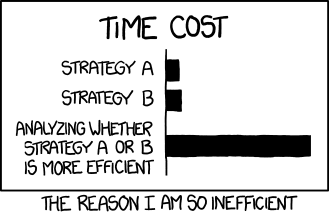
\includegraphics[height=0.6\textheight]{fig/xkcdefficiency}
\end{frame}


\begin{frame}{Profiling}
    \begin{definition}
        \structure{Profiling}: identify performance bottlenecks by measuring
    \end{definition}
    
    Two important measurements:
    \begin{itemize}
        \item How often is each function called
        \item How long does it take?
    \end{itemize}

    \pause\vspace{1em}
    Consider two scenarios:
    \begin{enumerate}
        \item A 100x speedup of a component responsible for 1\% of total runtime.
        \item A 1.1x speedup of a component responsible for 90\% of total runtime.
    \end{enumerate}
    Do not waste your time on 1; therefore: measure!
\end{frame}

\begin{frame}{Is it worth the time?}
    \begin{reference}\scriptsize\vspace{1em}
        \url{https://www.xkcd.com/1205/}
    \end{reference}
    \hfill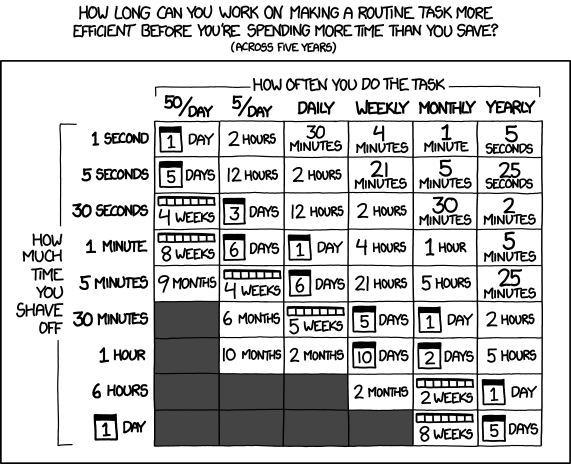
\includegraphics[height=0.9\textheight]{fig/xkcdworththetime}
\end{frame}

\begin{frame}{Takeaway}
    ``We should forget about small efficiencies, say about 97\% of the time:
    premature optimization is the root of all evil. Yet we should not pass up
    our opportunities in the critical 3\%'' -- Donald Knuth

    \vspace{1em}
    \begin{itemize}
        \item Consider expected return on investment
        \item Optimization risks overcomplicating \& over-engineering
    \end{itemize}
\end{frame}

\begin{frame}{Summary}
    Improving code involves
    \begin{itemize}
        \item Debugging
        \item Re-factoring, code style
        \item Optimization, profiling
    \end{itemize}
\end{frame}



% break


\section{Sentiment analysis}
\subsection{Identifying positive and negative language}
\frame{\tableofcontents[currentsection]}

\begin{frame}{Sentiment analysis}
    \begin{definition}
        \structure{Sentiment (polarity) analysis}: 
            is a piece of language positive or negative?
    \end{definition}

    Applications:
    \begin{itemize}
        \item Identify positive/negative reviews
        \item Monitor complaints about a company on social media
    \end{itemize}

    \pause
    How to estimate?
    \begin{itemize}
        \item Create sentiment word lists
        \item Assign each word a score, e.g.: \\
            negative vs positive, 5-point scale, etc.
        \item Positive: good, swell, benevolent, admire, etc. \\
                Negative: bad, sour, abnormal, hinder, etc.
        \item Combine scores for each word into a total score. \\
                (simple sum, or train classification model)
    \end{itemize}
\end{frame}

\begin{frame}{Challenges}
    Can we really reduce sentiment to counts of positive/negative words?

    \begin{itemize}
        \item Negation
        \item Polysemy
        \item Non-literal meaning
        \item etc. etc.
    \end{itemize}

    Still, the `stupid' model works surprisingly well.

    Many tricks for minor improvements.
\end{frame}

\begin{frame}[fragile]{Sentiment word counting in Python}
    \begin{reference}\scriptsize
        Word lists: \url{https://www.kaggle.com/rtatman/sentiment-lexicons-for-81-languages} \\
        Proper sentiment analysis: \url{https://www.twilio.com/blog/2017/12/sentiment-analysis-scikit-learn.html}
        % \https://stackabuse.com/python-for-nlp-sentiment-analysis-with-scikit-learn/}
        %\url{https://towardsdatascience.com/basic-binary-sentiment-analysis-using-nltk-c94ba17ae386}
        % Issues: uses NLTK's classifiers / API.
        % \url{https://nealcaren.org/lessons/wordlists/}
        % Issues: uses Pandas, relies on installing package w/sentiment lexicon;
        % no classifier
        %\url{http://www.nltk.org/howto/sentiment.html}
        % issues: NLTK classifiers, no explanation
    \end{reference}
\begin{lstlisting}
import nltk
from collections import Counter
with open('data/sentiment/positive.txt') as inp:
    positive_words = set(inp.read().splitlines())
with open('data/sentiment/negative.txt') as inp:
    negative_words = set(inp.read().splitlines())
with open('VERNE, Jules - A Journey to the Center of the Earth.txt') as inp:
    tokens = nltk.word_tokenize(inp.read().lower())
counts = Counter(tokens)
sentiment = 0
for word, count in counts.items():
    if word in positive_words:
        sentiment += count
    elif word in negative_words:
        sentiment -= count
\end{lstlisting}
\end{frame}

\subsection{Does every story reduce to six basic plot shapes?}
% Show other/simpler example applications in literature?
\begin{frame}{Kurt Vonnegut: The simple shapes of stories}
    \begin{reference}
        More information:
        \url{https://www.brainpickings.org/2012/11/26/kurt-vonnegut-on-the-shapes-of-stories/}
    \end{reference}
    \begin{columns}
        \column{0.5\linewidth}
    \centering\large
    \url{https://youtu.be/oP3c1h8v2ZQ?t=20}
        \column{0.5\linewidth}\centering
        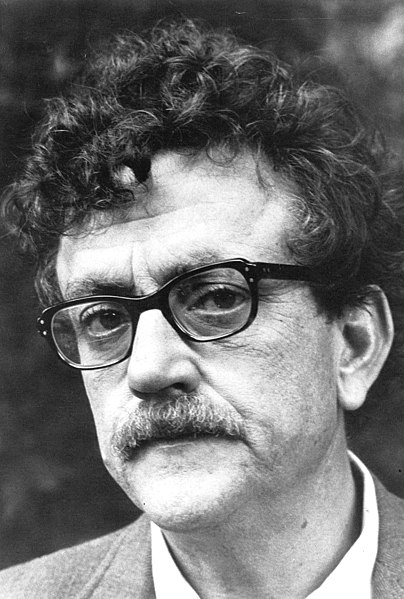
\includegraphics[height=0.5\textheight]{fig/vonnegut}
    \end{columns}
\end{frame}

\begin{frame}{Can we operationalize this?}
    \begin{reference}
        Matthew Jockers (2015) \url{http://www.matthewjockers.net/2015/02/02/syuzhet/} \\
        Reagan et al (2015) \url{https://doi.org/10.1140/epjds/s13688-016-0093-1}
    \end{reference}
    Yes we can!
    
    \begin{columns}
        \column{0.5\linewidth}
    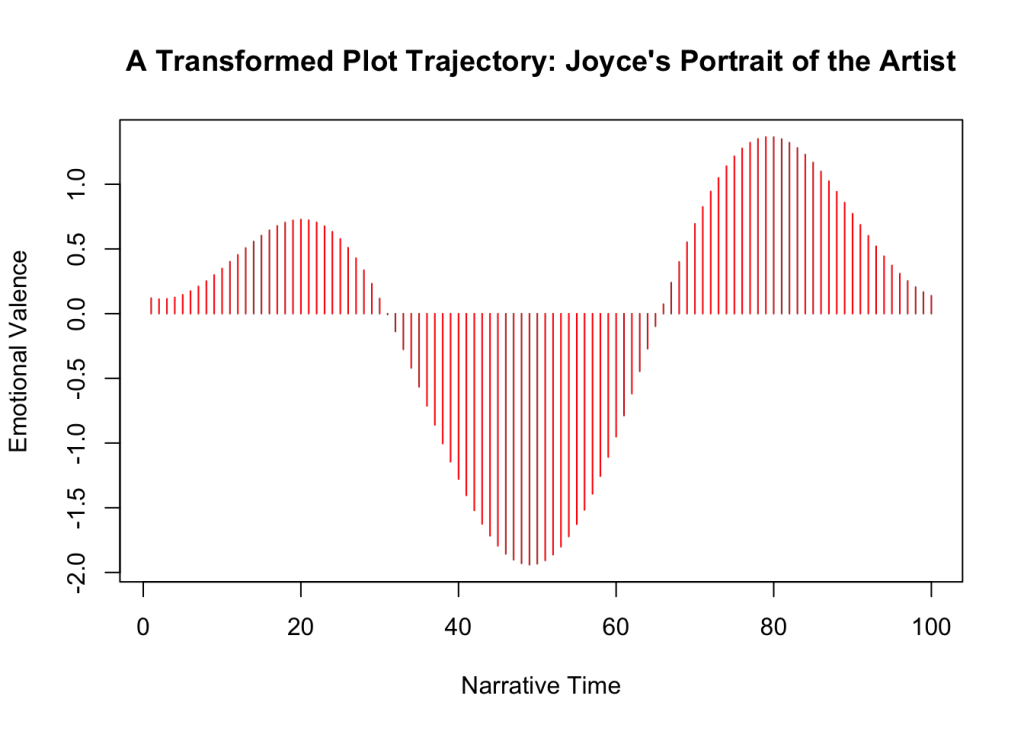
\includegraphics[width=1\textwidth]{fig/joycearc}

        \column{0.5\linewidth}
    \begin{itemize}
        \item Estimate emotions: count sentiment words
        \item Chop text into chunks of x words, count sentiment in each chunk
        \item Recognize plot shapes: SVD / Fourier transform
    \end{itemize}
    \end{columns}
    Seems to confirm that all novels have a few basic story shapes!
\end{frame}

\begin{frame}{But \dots Hold your horses!}
    \begin{reference}
        \url{https://annieswafford.wordpress.com/2015/03/07/continuingsyuzhet/} \\
        \url{https://senderle.github.io/svd-noise/}
    \end{reference}

    \begin{columns}
        \column{0.5\linewidth}
            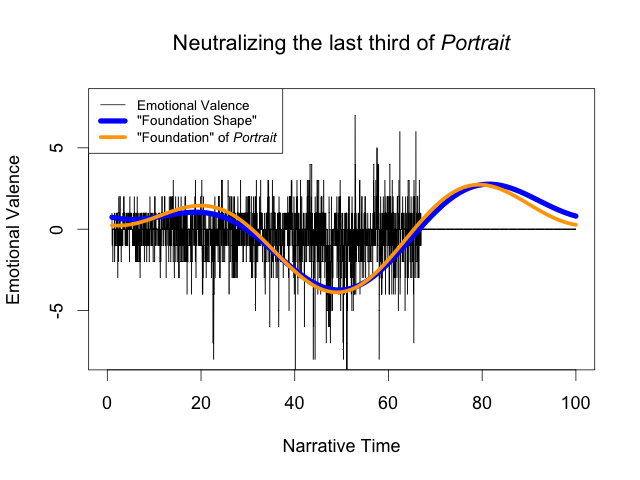
\includegraphics[width=0.9\linewidth]{fig/joycenoise}
        \column{0.5\linewidth}
    \begin{itemize}
        \item Reducing \structure{emotions} to binary sentiment word frequencies \\
            is naive \& crude
        \item The reduction to basic story shapes appears to be \\
            a reflection of noise and artefacts.
    \end{itemize}
    \end{columns}

    \pause
    Takeaway:
    \begin{itemize}
        \item Yes, if you insist, you can reduce anything to 6 story shapes \\
            (or 3, 10, 100, etc.)
        \item No, this does not appear to be enlightening.
    \end{itemize}
\end{frame}

\begin{frame}{Summary}
    \begin{itemize}
        \item Sentiment in text can be measured
        \item Interesting patterns may emerge; but caveat emptor
    \end{itemize}
\end{frame}



\section{Keyword analysis}
\subsection{Keywords in context with NLTK}
\frame{\tableofcontents[currentsection]}

\begin{frame}[fragile]{NLTK: explore keywords in context}
    \begin{reference}
        \url{https://www.nltk.org/book/ch01.html}
    \end{reference}
    NLTK \texttt{Text} object offers:
    \begin{itemize}
        \item Concordance
        \item Similar words
        \item Common contexts
        \item Collocations
        \item Dispersion plot
    \end{itemize}
Make \texttt{Text} objects:
\begin{lstlisting}
In: import nltk
In: with open('MELVILLE, Herman - Moby Dick.txt') as inp:
...     moby_dick = nltk.Text(nltk.word_tokenize(inp.read()))
In: with open('AUSTEN, Jane - Sense and Sensibility.txt'):
...     austen_sense = nltk.Text(nltk.word_tokenize(inp.read()))
\end{lstlisting}
\end{frame}

\begin{frame}[fragile]{Concordance}
\begin{lstlisting}
In: moby_dick.concordance('monstrous')
\end{lstlisting}
\begin{lstlisting}[style=plain]
Ho ' s Story . CHAPTER 55 . Of the Monstrous Pictures of Whales . CHAPTER 56 .
ong the former , one was of a most monstrous size ... . This came towards us ,
n of the Psalms_ . " Touching that monstrous bulk of the whale or ork we have r
ll over with a heathenish array of monstrous clubs and spears . Some were thick
d as you gazed , and wondered what monstrous cannibal and savage could ever hav
that has survived the flood ; most monstrous and most mountainous ! That Himmal
they might scout at Moby Dick as a monstrous fable , or still worse and more de
of Radney. ' " CHAPTER 55 . Of the Monstrous Pictures of Whales . I shall ere l
ing Scenes . In connexion with the monstrous pictures of whales , I am strongly
ere to enter upon those still more monstrous stories of them which are to be fo
ght have been rummaged out of this monstrous cabinet there is no telling . But
e of Whale-Bones ; for Whales of a monstrous size are oftentimes cast up dead u
\end{lstlisting}
\end{frame}

\begin{frame}[fragile]{Similar words}
\begin{lstlisting}
In: moby_dick.similar("monstrous")
\end{lstlisting}
\begin{lstlisting}[style=plain]
mean part maddens doleful gamesome subtly uncommon careful untoward
exasperate loving passing mouldy christian few true mystifying
imperial modifies contemptible
\end{lstlisting}
\begin{lstlisting}
In: austen_sense.similar("monstrous")
\end{lstlisting}
\begin{lstlisting}[style=plain]
very heartily so exceedingly remarkably as vast a great amazingly
extremely good sweet
\end{lstlisting}

\structure{Insight}: monstrous is positive for Austen!
\end{frame}

\begin{frame}[fragile]{Common contexts}
\begin{lstlisting}
In [6]: austen_sense.common_contexts(['monstrous', 'very'])
\end{lstlisting}
\begin{lstlisting}[style=plain]
a_pretty am_glad a_lucky is_pretty, be_glad
\end{lstlisting}

\pause
i.e., Sense \& Sensibility contains both ``a very pretty" \\
    and ``a monstrous pretty" etc.

\begin{lstlisting}
In: austen_sense.concordance('monstrous')
\end{lstlisting}
\begin{lstlisting}[style=plain]
Displaying 11 of 11 matches:
 `` Now , Palmer , you shall see a monstrous pretty girl . '' He immediately we
your sister is to marry him . I am monstrous glad of it , for then I shall have
[...]
\end{lstlisting}
\end{frame}

\begin{frame}[fragile]{Collocations}
\begin{definition}
    A \structure{collocation} is a sequence of words that occur together
    unusually often. Thus \emph{red wine} is a collocation,
    whereas \emph{the wine} is not. (source: NLTK book)
\end{definition}
\begin{lstlisting}
In: moby_dick.collocations()
\end{lstlisting}
\begin{lstlisting}[style=plain]
Sperm Whale; Moby Dick; White Whale; old man; Right Whale; Captain
Ahab; sperm whale; New Bedford; Captain Peleg; Mr. Starbuck; Cape
Horn; cried Ahab; Mrs. Hussey; years ago; chief mate; lower jaw;
Father Mapple; white whale; ivory leg; cried Stubb
\end{lstlisting}
\begin{lstlisting}
In: austen_sense.collocations()
\end{lstlisting}
\begin{lstlisting}[style=plain]
Mrs. Jennings; Colonel Brandon; Sir John; Lady Middleton; Mrs.
Dashwood; Miss Dashwood; Mrs. Ferrars; every thing; thousand pounds;
dare say; Mr. Palmer; Miss Steeles; said Elinor; Mrs. Palmer; Miss
Steele; every body; Mr. Willoughby; John Dashwood; great deal; Harley Street
\end{lstlisting}
\end{frame}

\begin{frame}[fragile]{Dispersion plot}
\begin{lstlisting}
%matplotlib inline
moby_dick.dispersion_plot(['whale', 'ship'])
\end{lstlisting}

    \centering
    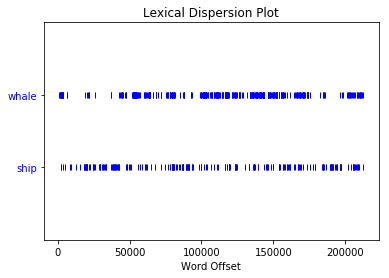
\includegraphics[height=0.6\textheight]{fig/dispersion}
\end{frame}

% move on to scikit-learn / pandas for extracting keywords with statistics
\subsection{Discovering distinctive keywords}
\begin{frame}{Distinctive words}
    Finding statistically characteristic words in a text:
    \begin{itemize}
        \item Identify important topics (content words)
        \item Identify stylistic characteristics (function words)
        \item Contrast two (sets of) texts (keyness)
    \end{itemize}

    Keyword selection methods:
    \begin{itemize}
        \item Simple word frequency
        \item Chi-square
        \item tf-idf
    \end{itemize}

    % Example applications in DH?
\end{frame}

\begin{frame}[fragile]{Why not normal frequencies?}
\begin{lstlisting}
In: moby_dick.vocab()
Out: FreqDist({'the': 13694, 'of': 6531, 'and': 5932, 'a': 4493, 'to': 4459,
    'in': 3850, 'that': 2679, 'his': 2428, 'I': 1723, 'with': 1649, ...})

In: austen_sense.vocab()
Out: FreqDist({'to': 4010, 'the': 3847, 'of': 3535, 'and': 3191, 'her': 2135,
    'a': 1996, 'in': 1833, 'was': 1773, 'I': 1673, 'she': 1257, ...})
\end{lstlisting}

\begin{itemize}
    \item The most frequent words are function words (up to, say, 50 words).
    \item Informative about style and authorship.
        \url{https://programminghistorian.org/en/lessons/introduction-to-stylometry-with-python}
    \item Mostly pretty similar and uninformative about content.
    \item Simple solution: throw away frequent ``stop words''
\end{itemize}
\end{frame}

\begin{frame}[fragile]{Chi-square: Most distinctive words in two sets of texts}
    \begin{reference}
        \url{http://www.thegrammarlab.com/?nor-portfolio=understanding-keyness} \\
        \url{https://liferay.de.dariah.eu/tatom/feature_selection.html}
    \end{reference}
% issues: uses numpy, pandas, scikit-learn
\begin{lstlisting}
import numpy as np
from sklearn.feature_extraction.text import CountVectorizer
from sklearn.feature_selection import chi2
filenames = ['MELVILLE, Herman - Moby Dick.txt',
        'AUSTEN, Jane - Sense and Sensibility.txt']
vectorizer = CountVectorizer(input='filename')
document_term_matrix = vectorizer.fit_transform(filenames)
vocab = np.array(vectorizer.get_feature_names())
labels = filenames  # use to distinguish the sets
keyness, pvalues = chi2(document_term_matrix, labels)
ranking = np.argsort(keyness)[::-1]
vocab[ranking][0:10]
\end{lstlisting}
Result:
\begin{lstlisting}
['the', 'her', 'she', 'whale', 'of', 'and', 'in', 'elinor', 'his', 'that']
\end{lstlisting}
\end{frame}

\begin{frame}[fragile]{tf-idf}
\begin{reference}\scriptsize
    \url{https://suzil.ai/2019/01/15/extract-keywords-from-text-snippets-using-tfidf-and-sklearn/}
    % issues: uses numpy, pandas, scikit-learn
    \url{https://programminghistorian.org/en/lessons/analyzing-documents-with-tfidf}
\end{reference}
tf-idf = term frequency / document frequency

    \begin{itemize}
        \item Intuition: compare frequencies against background corpus.\\
            Look for words with the largest contrast in frequency.
        \item Finds good topical words: what is unique about this document?
        \item Only works if you have a large number of documents! \\
            (i.e., large corpus, say 100+ texts)
        \item Example application: automatically adding ``tags'' \\
            to social media posts
    \end{itemize}
\end{frame}

\begin{frame}{Summary}
    \begin{itemize}
        \item Searching keywords
        \item Discovering keywords
    \end{itemize}
\end{frame}

% \begin{frame}{Mini-project}
%     \structure{Proposal}:
%     \begin{itemize}
%         \item Mini-project instead of take-home exam.
%         \item Same deadline, start now, work individually
%         \item Pick text analysis method (sentiment analysis, keyword analysis)
%         \item Pick dataset from your field (a few options will be made available)
%         \item Think of a simple (answerable) research question
%         \item \structure{Hand in}:
%             Notebook with code, quantitative results, interpretation,
%             and discussion.
%     \end{itemize}
% \end{frame}

\begin{frame}{Background reading}
    See all the links on the slides \dots (clickable)
\end{frame}

\end{document}
